%\documentclass[rmp,twocolumn]{revtex4}
\documentclass[rmp]{revtex4}
\usepackage[english]{babel}
\usepackage{amssymb,amsfonts,amsmath}
\usepackage{color}
\usepackage{breqn}
\usepackage{graphicx}
\usepackage{caption}
\usepackage{subcaption}
\captionsetup{compatibility=false}

\usepackage{amsmath}
\usepackage{natbib}
\usepackage{hyperref}
\usepackage{enumerate}
%\usepackage{subfig}

% Code syntax highlighting
\usepackage{listings}
\lstloadlanguages{C++,Python}

\newcommand{\EQ}[1]{Eq.~(\ref{eq:#1})}
\newcommand{\EQS}[2]{Eqs.~(\ref{eq:#1}) and (\ref{eq:#2})}
\newcommand{\FIG}[1]{Fig.~\ref{fig:#1}}
\newcommand{\TAB}[1]{Tab.~\ref{tab:#1}}
\newcommand{\REF}[1]{ref.~\citep{#1}}

\newcommand{\comment}[1]{{\color{red}#1}}

\definecolor{dkgreen}{rgb}{0,0.6,0}
\definecolor{gray}{rgb}{0.5,0.5,0.5}
\definecolor{mauve}{rgb}{0.58,0,0.42}

\DeclareMathOperator*{\argmin}{arg\,min}

%%%%%%%%%%%%%%%%%%%%%%%%%%%%%%%%%%%%%%%%%%%%%%%%%%%%%%%%%%%%%%%%%%%%%%%%%%%%%%
\begin{document}
%%%%%%%%%%%%%%%%%%%%%%%%%%%%%%%%%%%%%%%%%%%%%%%%%%%%%%%%%%%%%%%%%%%%%%%%%%%%%%
\title{Genetic draft and the evolution of ``irreducible complexity"}
\author{Taylor~Kessinger}
\author{Jeremy~Van~Cleve}
%\affiliation{Department of Biology, University of Kentucky}


\date{\today}

%%%%%%%%%%%%%%%%%%%%%%%%%%%%%%%%%%%%%%%%%%%%%%%%%%%%%%%%%%%%%%%%%%%%%%%%%%%%%%
\begin{abstract}

Living systems are characterized by complex adaptations, at least some of which have arisen by evolutionary paths whose intermediate states are neutral or even deleterious.
Such adaptations have been termed ``irreducibly complex", and the process by which they evolve is known as ``crossing a fitness valley".
Previous efforts have rigorously characterized the rate at which such complex adaptations evolve in populations of roughly equally fit individuals.
However, populations that are very large or have broad fitness distributions, such as many microbial populations, adapt quickly, which substantially alters the fate of individual mutations.
We investigate the rate at which irreducible complexity evolves in these rapidly adapting populations, focusing on asexual populations.
We confirm that rapid adaptation overall increases the time required to cross a valley but can make it easier for deeper valleys to be crossed.
\end{abstract}

\maketitle

\section*{Introduction}

The simplest adaptive scenarios in evolution involve the arisal and fixation of successive beneficial mutations.
This appears to be how Darwin thought most complex systems, such as the vertebrate eye, evolved \citep{darwin_1859}, and this assumption underlies much of the field of adaptive dynamics.
However, many adaptations exist that do not appear to have formed by this process.
One class of such adaptations has been termed ``irreducibly complex" because, in their current forms, they cease to function when one or more of their parts is removed.
\citet{muller_1918} described one method by which such adaptations could evolve: components that originally served independent functions might become dependent on each other, giving the appearance of irreducibility.
An alternate method comes from the metaphor of a ``fitness landscape": a wild type individual must traverse a lower fitness mutational ``valley" in order to reach a higher fitness ``peak".
We seek to characterize this ``valley crossing" process, as there is reason to think it may in fact be a common mode of adaptation \citep{trotter_2014}.

Valley crossing in asexual populations is increasingly well understood \citep{weissman_2009}.
If the number of mutants produced every generation is high, the arisal of a complex adaptation that is destined to fix may be guaranteed.
In small populations, wild type individuals may give rise to neutral or deleterious intermediate mutants, which drift to fixation.
A third possibility is for wild type individuals to birth mutant ``bubbles", or transient subpopulations.
These bubbles are ordinarily doomed to extinction due to drift, but a lucky bubble may give rise to a complex adaptation that sweeps to fixation; this process has been referred to as ``tunneling" \citep{iwasa_2004, weissman_2009}.
These phenomena were successfully extended to sexually reproducing populations by \citet{weissman_2010}, which found that the criterion $r < s$, with $r$ the recombination rate and $s$ the selective advantage of the complex adaptation, is the necessary criterion for recombination to be helpful in crossing a valley.
Fairly low recombination rates can bring mutant subpopulations together, increasing the rate at which complex adaptations arise and sweep.
High recombination rates, on the other hand, lower the valley crossing rate by forcing fit individuals to outcross with the less fit wild type.

Previous studies of valley crossing focused primarily on populations where the background fitness variation is small enough to be negligible.
In these populations, genetic drift governs the fate of neutral alleles, as well as the behavior of deleterious or beneficial alleles close to frequency zero or one.
When population sizes are very large or the fitness variation in the population is substantial, however, the behavior of genetic variation is governed more by genetic \emph{draft} than by drift.
In a drafting asexual population, the fate of an allele depends sharply on its genetic background.
Only a handful of individuals near the ``nose" of the fitness distribution are likely to persist, and they give rise to the bulk of the future population, carrying linked alleles with them.
In sexual populations, much the same description applies.
The parameter that determines whether drift or draft is more important is the product of the population size $N$ and the standard deviation in fitness $\sigma$ \citep{neher_hallatschek_2013} or, in a sexual population, the proportion of fitness variation $\sigma_b$ that segregates within an effectively asexual block length \citep{neher_kessinger_2013}.

Drift and draft are fundamentally different forces.
It is not possible to understand a drafting population in terms of a drifting one, for example by defining a reduced ``effective population size".
Drafting populations do not admit a diffusion approximation, and they exhibit qualitatively different genealogies and site frequency spectra relative to a drifting population.
In fact, the possibility that neutral variants are affected more strongly by selection at linked sites than by genetic drift, even in organisms like \emph{Drosophila}, is one possible explanation for the ``paradox of variation", the fact that genetic diversity and population size often do not scale linearly.
Draft likewise has profoundly different effects on the evolution of complex adaptations.
\citet{neher_shraiman_2011} explored the dynamics of stochastic tunneling in rapidly adapting sexual populations.
The primary mode of recombination considered therein is ``free" recombination, in which parents essentially shuffle the entirety of their genomes during reproduction.
We extend this to asexual populations and comment on alternate modes of recombination, such as crossovers.
Using analytical approaches and forward simulations, we confirm that fitness valley crossing occurs at an overall lower rate in rapidly adapting populations, but that much deeper valleys can be crossed.
These observations add to the growing intuition that irreducible complexity may not be a surprising result of the evolutionary process, but rather an expected one.

\section*{Model}

Our model features a population of $N$ haploid individuals in which an effectively infinite number of ``background" loci, with weak fitness effects, are currently segregating.
We focus on two loci, which are initially fixed for alleles $a$ and $b$.
These alleles mutate to $A$ and $B$ at rates $\mu_a$ and $\mu_b$, respectively (we neglect back mutations).
Genotypes $ab$, $Ab$, $aB$, and $AB$ have fitnesses $1$, $1-\delta_a$, $1-\delta_b$, and $1+s$ respectively, with $\delta \geq 0$ (so the intermediate genotypes are deleterious) and $1/N < s < 1$ (so the complex adaptation is strongly beneficial).
For the remainder of our analysis, we will assume that $\mu_a = \mu_b$ and $\delta_a = \delta_b$: we discuss the effects of relaxing this assumption in the appendix.
We further assume that the large number of loci of weak effect contribute to a background fitness variance $\sigma^2$ which, by Fisher's ``fundamental theorem" of natural selection, sets the rate at which the mean fitness advances.
Let $x$ be the background fitness of a lineage.
The distribution of background fitnesses $f(x)$ is assumed to be roughly Gaussian: $f(x) = \frac{1}{\sqrt{2\pi}\sigma} \exp (\frac{(x-\bar{x})^2}{2\sigma^2})$.
Our goal is to compute the expected time $\mathbb{E}\left[ T\right]$ for such a complex adaptation to arise and fix in the population, as a function of the parameters.

In very large populations, enough double mutants are generated that the valley crossing time is dominated by the time required for a selective sweep to occur.
At the other extreme, in small populations, the crossing time is dominated by the wait for a deleterious single mutant to fix: only thereafter does a successful double mutant appear.
We begin by zeroing in on the intermediate case: stochastic tunneling, the most interesting and mathematically demanding mode of valley crossing.
Once this is understood, extending our results to incorporate sequential fixation or the arisal of a complex adaptation in a single generation is straightforward.

There are essentially three components to this process.
First, a single mutant lineage must appear, which occurs with rate $N\mu$.
During the lifetime of this mutant lineage, the complex adaptation must appear and establish, that is, rise to a high enough frequency that fixation is almost guaranteed, which occurs at rate $\mu p_{\mathrm fix}$.
Finally, the complex adaptation must sweep to fixation.
The first two steps can be folded in together and considered as one process, so that what is relevant is the expected time until a single mutant lineage arises that is destined to produce a successful double mutant.
In this way, $\mathbb{E}\left[ T \right] = \mathbb{E} \left[ T_0 + T_1 \right]$, where $T_0$ is the time to the first successful bubble and $T_1$ is the sweep time.
We assume that $T_0 \gg T_1$, so that the wait time is dominated by the first term.

We refer to single mutant lineages as ``bubbles".
Let $n(t)$ be the total number of single mutant individuals in the bubble, and suppose it appears at time $t_0$ and goes extinct at time $T$.
Then $W = \int_{t_0}^T n(t)dt$ is the ``weight" of the bubble, representing the total number of chances there are for a successful double mutant to appear.
Most of the time, a bubble will simply arise and go extinct.
However, with probability $1-e^{-\mu p_{\mathrm fix} W}$, the bubble will give rise to a successful double mutant.
Computing the expected value $\phi = \left< 1-e^{\mu p_{\mathrm fix} W} \right>$ thus gives the probability that a particular bubble will lead to a successful valley crossing.

One difficulty in computing the rate of tunneling in the high $N\sigma$ case is that the expected bubble size and fixation probability will both turn out to depend on the background fitness of an individual.
That is to say, one cannot simply compute $p_{\mathrm{fix}}$ and the weight distribution by themselves but rather must convolute both of them over the background fitness.
Individuals near the nose of the distribution will tend to give rise to longer-lived lineages, and because they are near the nose, the complex adaptation will therefore likewise be more likely to fix.
As a result, $W$ will depend on $x$ and $\delta$, and $p_{\mathrm fix}$ will depend on $x$ and $s$.
These will have to be integrated over the fitness distribution $f(x)$ in order to obtain the total crossing probability $\Phi(s,\delta) = \int_{-\infty}^\infty \phi(x,s,\delta) f(x) dx$.
The expected valley crossing time then becomes $1/N\mu\Phi$.


We begin by considering the dynamics of $p_{\mathrm fix}$ before moving on to consider the distribution of bubble sizes.
Let $p = p_{\mathrm fix}(x,s,t)$ be the fixation probability of the double mutant as a function of the absolute fitness $x$.
In the absence of any perturbations, the evolution of $p$ can be described by a birth-death process, yielding
\begin{equation}
-\partial_t p(x,s,t) = Bp(x,s,t) - (B+D)p(x,s,t)^2
\end{equation}
\citep{barton_1995, good_2012}, with $B$ and $D$ the birth and death rates respectively.
The only dependence of $p$ on $t$ is via the time-changing mean fitness $vt$.
Defining $X = x - vt$, we then have $\partial_t p(x-vt) = -v\partial_X p(X)$.
This can be rewritten as a wave equation
\begin{equation}
v \partial_X p(X,s) = (X+s)p(X,s) - (1+X+s)p(X,s)^2.
\end{equation}
This is a Bernoulli equation and is readily solved, but the only appropriate boundary condition yields $p = 0$ everywhere.
This is intuitive: the inexorable advance of the mean fitness implies that all lineages are ultimately doomed to extinction \emph{unless} they can increase their own fitness either via recombination or mutation.
We thus need to amend the model to include a mutation term.
Let $U$ be the mutation rate of the genetic background and $\epsilon$ be the fitness effect of a mutation, distributed as $\rho(\epsilon)$.
Then we have
\begin{equation}
v \partial_X p(X,s) = (X+s)p(X,s) - (1+X+s)p(X,s)^2 + U\int_0^\infty \rho(\epsilon) \left[ p(X+\epsilon,s)-p(X,s)\right] d\epsilon,
\end{equation}
where $\epsilon$ is now the fitness effect of a mutation in the background distribution, $\rho(\epsilon)$ is the distribution of mutational effects, and $U$ is the mutation rate of the background.
Assuming that $s$ is small compared to $\sigma$, a matched asymptotics analysis yields
\begin{equation}
p(X,s) =
\begin{cases}
0 &\mathrm{~if~} X+s < 0, \\
X_c e^{\frac{(X+s)^2-X_c^2}{2\sigma^2}} &\mathrm{~if~} 0 < X+s < X_c, \\
X+s &\mathrm{~if~} X+s > X_c.
\end{cases}
\end{equation}
(If $s$ is large compared to $\sigma$, then the standard Haldane result, $p(s) \sim s$, obtains.)
Effectively, this means the fixation probability is \emph{zero} if the double mutant lineage's fitness is less than the average for the population: if the fitness is less than some critical value $X_c$, then the lineage must generate a background mutant in order to fix, and if it is above $X_c$, the fixation probability is determined by the lineage's ability to survive drift and establish.
The value of $X_c$ is determined by the shape of $\rho(\epsilon)$.
Suppose $\rho$ is distributed exponentially: $\rho(\epsilon) = \frac{1}{\bar{\epsilon}} e^{-\epsilon/\bar{\epsilon}}$.
Then $X_c$ is determined by solving
\begin{equation}
2 = \frac{\sqrt{2\pi}\sigma U}{\bar{\epsilon}} \left[ \frac{1}{X_c - \frac{\sigma^2}{\bar{\epsilon}}} + \frac{\bar{\epsilon}}{\sigma^2} \left( 1+ \frac{\bar{\epsilon}}{X_c} \right) \right] e^{\frac{(X_c - \sigma^2/\bar{\epsilon})^2}{2\sigma^2}}. 
\end{equation}

We now consider the behavior of single mutant bubbles.
Since the tunneling probability for a lineage with background fitness $x$ is given by $\phi = \left< 1 - e^{-\mu p_{\mathrm fix} W} \right>$, we do not need to compute the full distribution of $W$ but rather only its Laplace transform: $\mathcal{L}\left[ p(w) \right] = \int_0^\infty e^{-zw} p(w) dw$, with $z = \mu p_{\mathrm fix}$.
We proceed to derive an equation for the time evolution of the Laplace transform.

Let $p(w,T|k,t,x)$ be the probability that a bubble has reached weight $w$ at time $T$, given that there were $n$ individuals present in the lineage at time $t$, and the bubble has background fitness $x$.
We have
\begin{align*}
-(\partial_t -k\partial_w) p(w,T|k,t,x) = &-k(2+x-\bar{x}-\delta)p(w,T|k,t,x) \\
& + k(1+x-\bar{x}-\delta)p(w,T|k+1,t,x) \\
& +kp(w,T|k-1,t,x).
\end{align*}
Consider the Laplace transform $\mathcal{L}\left[ p(w,T|k,t,x) \right] = \hat{p}(z,T|k,t,x) =  \int_0^\infty e^{-zw} p(w,T|k,t,x) dw$.
Using the convolution property of the transform, as well as the fact that each lineage is independent, allows us to write $\hat{p}(w,T|k,t,x) = \hat{p}^k(w,T|1,t,x)$.
We therefore have
\begin{equation}
-\partial_t\hat{p}(z,T|t,x) = -z\hat{p}(z,T|t,x) -(2+x-\bar{x}-\delta)\hat{p}(z,T|t,x) + (1+x-\bar{x}-\delta)\hat{p}(z,T|t,x)^2 + 1.
\end{equation}
Defining $\phi = 1-\hat{p}$ (consistent with our previous definition of $\phi$ and normalizing our variables via $\tau = \sigma(T-t)$, $\chi = x/\sigma-\sigma T$, $\tilde{z} = z/\sigma$, and $\tilde{\delta} = \delta/\sigma$ yields
\begin{equation}
\partial_\tau \tilde{\phi} = \tilde{z} + (\tilde{z} + \chi + \tau + \tilde{\delta})\tilde{\phi} - (1 + \chi + \tau + \tilde{\delta})\tilde{\phi}^2,
\end{equation}
where $\tilde{\phi}$ = $\phi/\sigma$.
We assume that the prefactor of $\tilde{\phi}^2$ is approximately $1$, which corresponds to the growth rate being small compared to $1$.
In addition, we will eventually want to take the limit as $\tau \to \infty$, which corresponds to averaging over all possible bubble sizes, no matter how long lived they are.
However, this will yield the absurd result that $\tilde{\phi}$ grows without bound.
To remedy this, we assume that the lifespan of bubbles is short compared to the time scale over which selection acts, meaning that we drop the $\tau$ term.
Defining $\theta = \tilde{z} + \chi + \tilde{\delta}$ yields
\begin{equation}
\partial_\tau \tilde{\phi} = \tilde{z} + \theta \tilde{\phi} - \tilde{\phi}^2.
\end{equation}
Using matched asymptotics allows us to write
\begin{equation}
\tilde{\phi} = 
\begin{cases}
\tilde{z} &\mathrm{~if~} \theta < 0, \\
\theta &\mathrm{~if~} \theta > 0.
\end{cases}
\end{equation}
Intuitively, this corresponds to stating that bubbles with a positive growth rate are likely to persist for some time, but bubbles with a negative growth rate are doomed to extinction: the only way they can succeed is to generate a successful double mutant in $O(1)$ generations.
Knowing the form of $\phi$ and $z$ allows us to compute the overall tunneling probability and hence the expected time to a tunneling event, once we integrate over the fitness distribution $f(x)$.

%\begin{figure}
\begin{figure}
\begin{subfigure}[b]{0.4\textwidth}
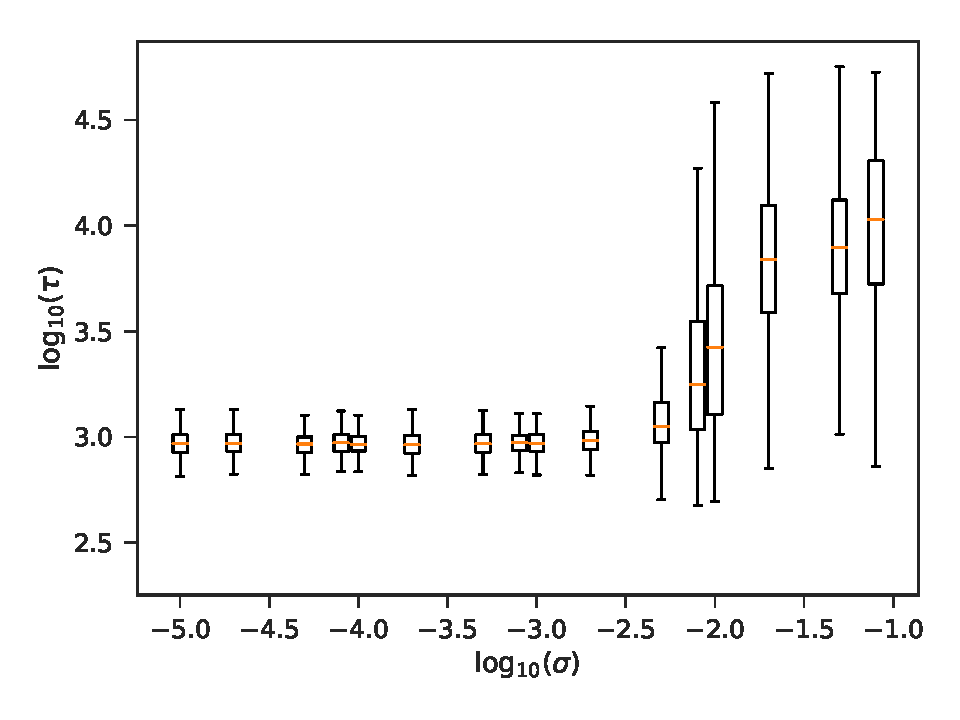
\includegraphics[width=\textwidth]{Figures/det_tunnel.pdf}
\end{subfigure}
\begin{subfigure}[b]{0.4\textwidth}
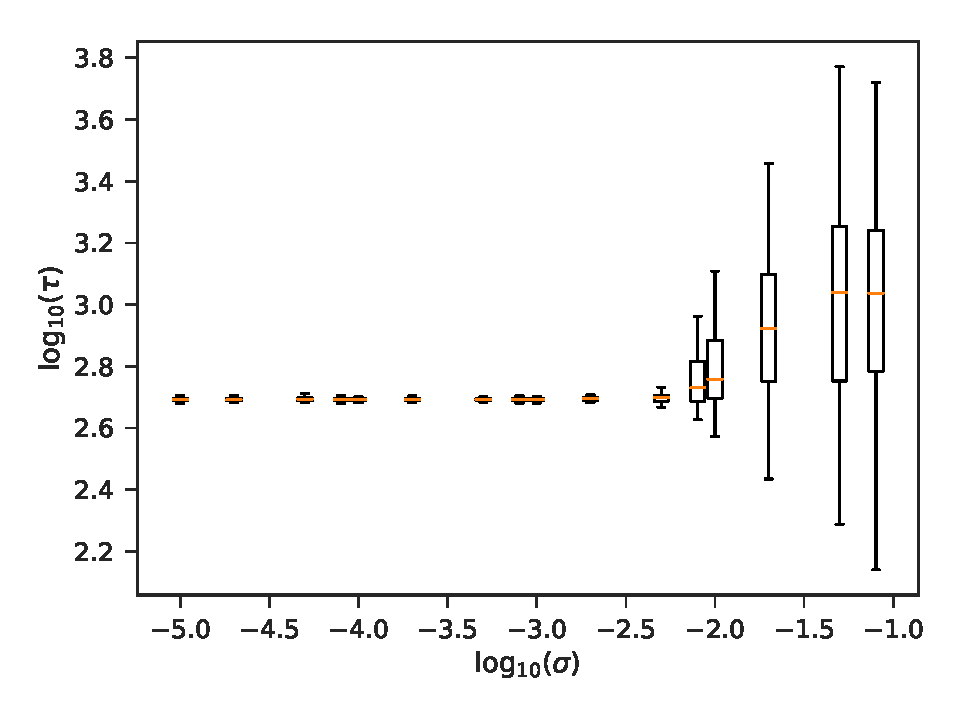
\includegraphics[width=\textwidth]{Figures/det_fix.pdf}
\end{subfigure}
\caption{Valley crossing times in the semi-deterministic tunneling (left) and deterministic fixation (right) regimes. In both figures, $s = 10^{-2}$ and $\delta = 10^{-3}$: on the left, $N = 10^5$ and $\mu = 10^{-4}$, and on the right, $N = 10^6$ and $\mu = 10^{-3}$. Orange lines are averages, boxes are interquartile ranges, and end caps are overall ranges. Each box represents about $100$ simulation runs.}
\label{fig:deterministic}
\end{figure}

\section*{Methods}

To test our model, we perform forward simulations using a customized version of \texttt{FFPopSim} \citep{zanini_2012}, a discrete time forward simulation package.
The simulation code is available from the authors upon request or via \texttt{GitHub}.
We initialize a wild type population of $N$ individuals consisting of haploid genomes of length $L = 200$.
For the genetic background, we make use of an \emph{ersatz} ``infinite sites" model, where any time a locus becomes monomorphic, a mutation is injected into a random individual in the population.
Background fitness effects are drawn from an exponential distribution, and the background fitness variance is set to a constant value $\sigma^2$ by manually adjusting the selection coefficients every generation.
In this way, $U$ and $\bar{\epsilon}$ are not parameters of our simulation model but must be directly measured from simulations: they are constrained by $L$ and $\sigma$.

We set the ``focal" loci (the loci at which the epistatic alleles segregate) to be at positions $L/4$ and $3L/4$.
Simulations are allowed to proceed for an ``equilibration" time of $N/10$ generations to allow sufficient genetic diversity to be introduced.
During this time, the mutation rate $\mu$ for the focal loci is set to zero.
After equilibration, we set a per-site mutation rate $\mu$ for the focal loci, with single mutant fitness disadvantage $\delta$ and double mutant advantage $s$, consistent with our analytical model.
When the double mutant reaches frequency $0.5$, we consider it to have fixed, then set the focal loci allele frequencies back to zero, randomize the selection coefficients for the genetic background, and allow the population to equilibrate for another $N/10$ generations.
This offers some assurance that independent valley crossing trials are indeed independent despite occurring in the same simulation run.
	
\section*{Results}

\begin{figure}
\begin{subfigure}[b]{0.4\textwidth}
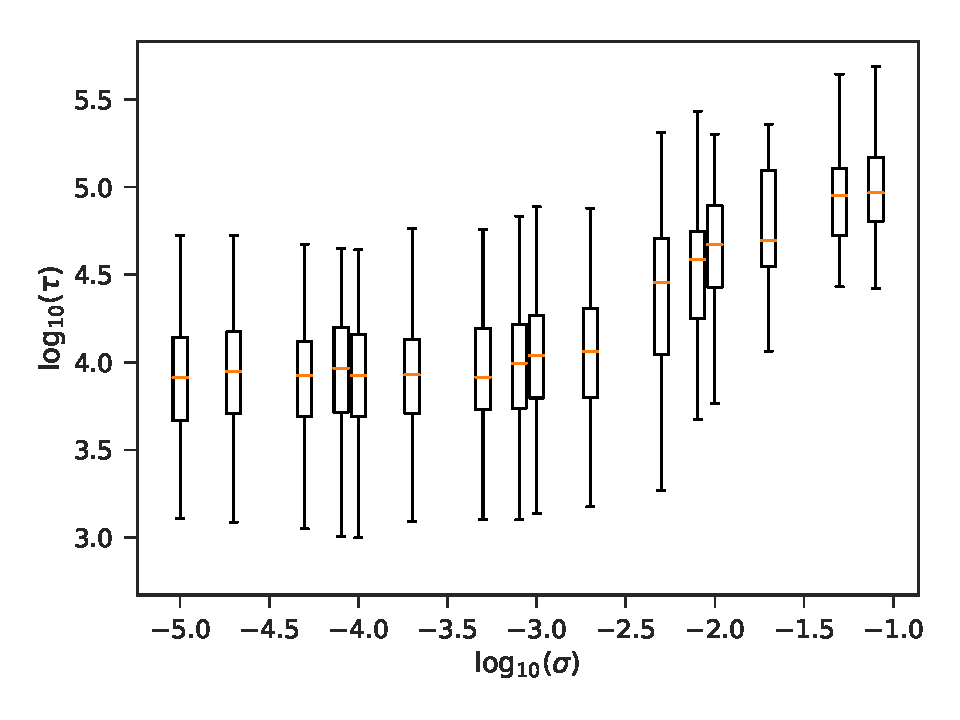
\includegraphics[width=\textwidth]{Figures/seq_fix.pdf}
\end{subfigure}
\begin{subfigure}[b]{0.4\textwidth}
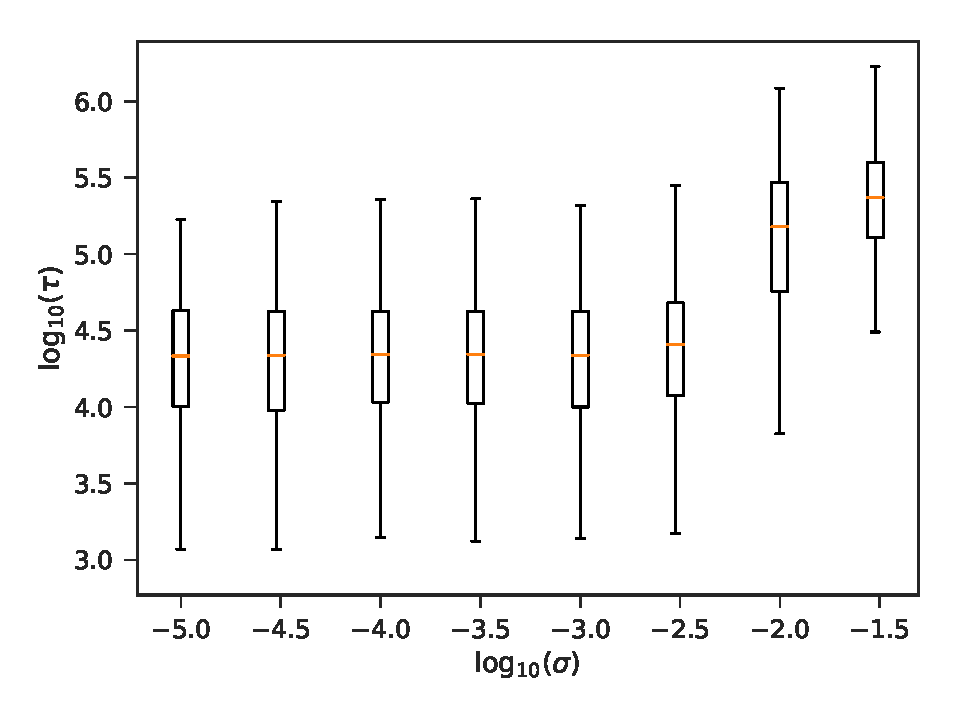
\includegraphics[width=\textwidth]{Figures/neut_tunnel.pdf}
\end{subfigure}
\caption{Valley crossing times in the sequential fixation (left) and tunneling (right) regimes. In both figures, $s = 10^{-2}$ and $\delta = 10^{-3}$: on the left, $N = 10^4$ and $\mu = 3\times 10^{-5}$, and on the right, $N = 10^5$ and $\mu = 3\times 10^{-6}$. Labeling is as in figure \ref{fig:deterministic}.}
\label{fig:tunneling}
\end{figure}

Here we present the key results of our simulation runs.
We first studied the effect of increasing $\sigma$ in what \citet{weissman_2009} describes as the sequential fixation, stochastic tunneling, semi-deterministic tunneling, and sequential fixation regimes.
Figures \ref{fig:deterministic} and \ref{fig:tunneling} show the expected result: the overall rate of valley crossing is generally slowed as $\sigma$ increases.
It is tempting to interpret this as a reduced $N_e$ due to a decrease in genetic diversity and the strength of selection.
The underlying dynamics are more complicated, however.
As $\sigma$ increases, the effect of the genetic background becomes more significant in determining the fate of an allele than the allele's fitness effect is.
The frequency of alleles is buffeted by genetic draft, so alleles behave as though they are more neutral than they really are.
This depresses the fixation probability of the complex adaptation, which appears to account for the majority of the change in fixation time.
In the case of stochastic tunneling, the overall size distribution of bubble sizes is reduced, as well: the distribution $P(w)$ scales not as $w^{-3/2}$ but as $w^{-2}$ \citep{neher_shraiman_2011}, so there are fewer chances for the complex adaptation to arise and fix.

\begin{figure}
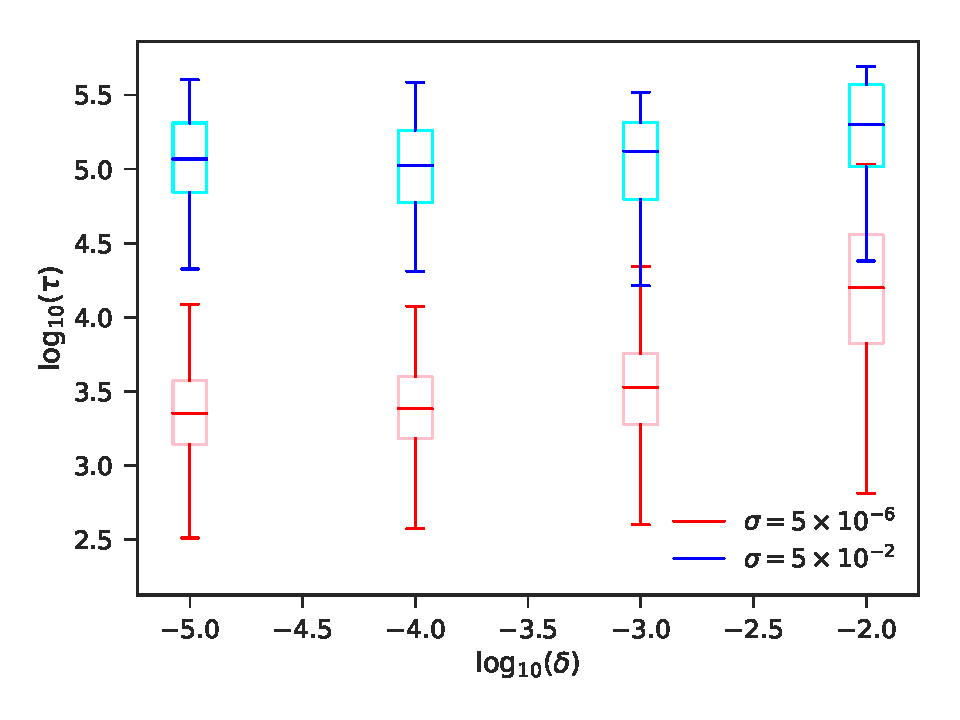
\includegraphics[width=0.4\textwidth]{Figures/var_sigma_delta.pdf}
\caption{Valley crossing times for varied $\sigma$ and $\delta$. In these simulations, $N = 10^5$, $\mu = 3 \times 10^{-6}$, and $s = 10^{-2}$. Note the lack of dependence on $\delta$ at high $\sigma$.}
\label{fig:sigma_delta}
\end{figure}

On the other hand, the reduced effectiveness of selection should generally be helpful in crossing deeper valleys, by mitigating the deleterious effect of single mutants.
This can be seen in figure \ref{fig:sigma_delta}.
At high values of $\sigma$, the fitness effect of the deleterious intermediate \emph{almost does not matter}, meaning that very deep valleys can be crossed.
This supports the view that traversing rugged fitness landscapes by valley crossing may be the rule, not the exception, in rapidly adapting populations.

\begin{figure}
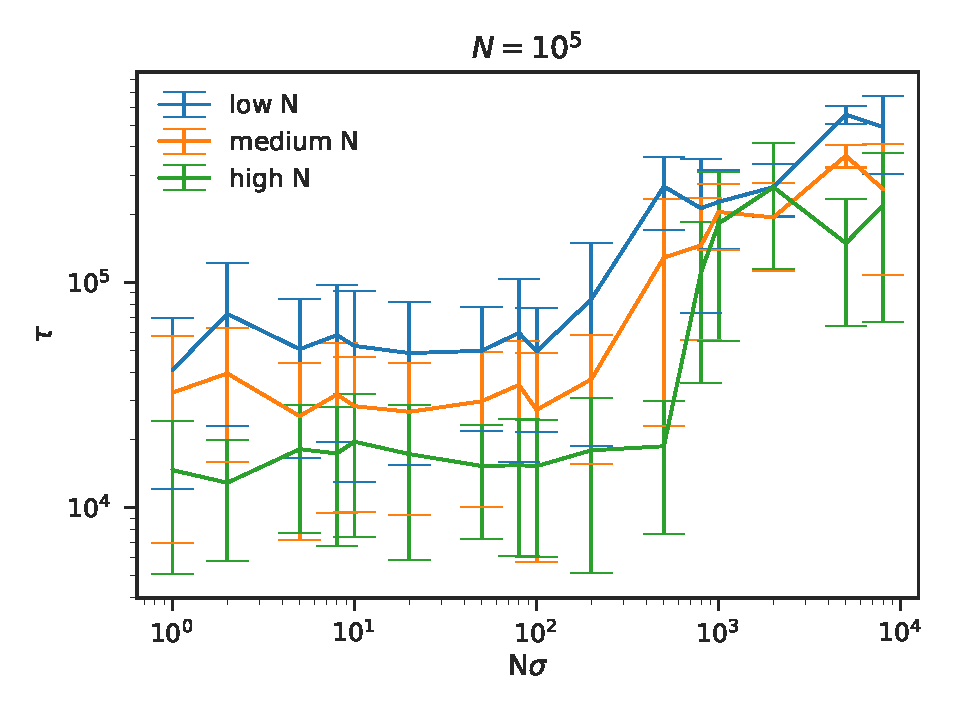
\includegraphics[width=0.4\textwidth]{Figures/bands.pdf}
\caption{Valley crossing times for fixed $N\sigma$, with $N$ allowed to vary up or down by a factor of $2$ (and $\sigma$ adjusted accordingly). Error bars are quartile ranges. Here, $\mu = 3 \times 10^{-6}$, $\delta = 10^{-3}$, and $s = 10^{-2}$.}
\label{fig:bands}
\end{figure}

Finally, we consider the effects of the compound parameter $N\sigma$, which has previously been shown to determine the coalescent behavior of populations \citep{neher_hallatschek_2013, neher_kessinger_2013}.
Figure \ref{fig:bands} suggests that, at high values of $\sigma$, the value of $N\sigma$ is more important than $N$ itself in determining the valley crossing rate.
The dependence on $N$ appears to be reduced, consistent with general features of very large, rapidly adapting populations.




%In the case where $\rho = 0$ and the fitness variance $\sigma^2$ is small ($N\sigma \ll 1$), the rate of valley crossing agrees with \citet{weissman_2009}: when $\rho > 0$, the rate agrees with \citet{weissman_2010}.
%This is because, provided that $N\sigma \ll 1$, genetic drift is the major evolutionary process affecting the frequency of deleterious intermediates, and the fixation probability of the complex adaptation simply scales with $s$.
%We turn to the regime where $N\sigma \gg 1$, meaning that draft is more important than drift, but the fixation probability of the full complex adaptation is suppressed.
%By the central limit theorem, the background loci create a background fitness wave whose shape is roughly Gaussian.
%We assume that the constant influx of weak effect beneficial mutations keeps the fitness variance $\sigma^2$ roughly constant.
%We sketch some heuristics in this limit before providing a more formal analysis.

\iffalse
First, we consider the case where $\rho = 0$ and focus on what \citet{weissman_2009} refer to as the process of ``stochastic tunneling", where $N\mu \ll 1$.
As we shall see, the results in the $\rho = 0$ and low $\rho$ limits can easily be extended to sexually recombining populations: moreover, understanding the rate of tunneling will allow us to easily examine the rate at which sequential fixation and deterministic fixation occur.
In stochastic tunneling, a deleterious intermediate arises (at rate $N\mu$), and its lineage persists over a short time $T$, forming a transient ``bubble".
If the number of individuals in the lineage is given by $n(t)$, then the total number of individuals in the ``bubble" is $w = \int_{t_0}^T n(t) dt$.
We refer to $w$ as the ``weight" of the bubble.
The overall rate of valley crossing becomes $1/N\mu p$, with $p$ the probability that a particular bubble will give rise to a successful double mutant.
Thus, given that a deleterious intermediate appears, it has $w$ ``chances" to generate a successful complex adaptation, which it does at rate $\sim \mu s$: double mutants arise at rate $\mu$ and have a probability $\sim s$ of fixing.
The probability of achieving a weight of at least $w$ scales as $1/\sqrt{w}$ (or, equivalently, $P(w) \sim w^{-3/2}$), meaning that with probability $\sqrt{\mu s}$, a bubble gives rise to a successful single mutant.
This probability drops off rapidly at $1/\delta^2$, so for higher values of $\delta$ (so called ``deleterious tunneling"), the rate at which new complex adaptations are generated starts to fall: the size of the mutant subpopulation is bounded from above by roughly $1/\delta$.

In the high $N\sigma$ regime, the argument is much the same, but the underlying dynamics are different.
In stark contrast to the drift case, the fate of a complex adaptation depends strongly on the fitness $x$ of the genetic background on which it appears.
Individuals with fitness lower than some critical fitness $x_c$ are almost guaranteed to go extinct.
This means the fixation probability of the complex adaptation no longer scales with $s$, and $P(w) \sim w^{-2}$ instead of $w^{-3/2}$, meaning that the probability of reaching weight $w$ is $\sim 1/w$.
However, individuals with higher fitnesses can be destined for fixation, even if they are carrying a significant load of deleterious mutations.
This means the dependence on $\delta$ is significantly lessened: even deep fitness valleys can be crossed by a rapid enough wave.
(Still needed: expression for fixation probability of beneficial mutant--this should be easy enough to obtain.
Can start with equation 3 of \citet{neher_shraiman_2011} and drop the recombination term, which is what I'm doing now.
This is tantamount to a ``mean field" approximation but might still work out okay.
Other possible approach is to use something like the expression of  \citet{desai_fisher_2007} for the fixation probability and rescale it to a traveling wave model.
Once we have the fixation probability, studying sequential and deterministic fixation will be easier than studying tunneling, since sequential fixation is essentially two different fixation events.)

One difficulty in computing the rate of tunneling in the high $N\sigma$ case is that the expected bubble size and fixation probability will both turn out to depend on the background fitness of an individual.
That is to say, the total rate of valley crossing will be given by $\int P(x) p_{\mathrm{fix}}(x,s) \mathbb{E}\left[ w(x,\delta) \right] dx$, with $P(x)$ the (presumably Gaussian) background fitness distribution.
One cannot simply compute $p_{\mathrm{fix}}$ and the weight distribution by themselves but rather must convolute both of them over the background fitness.
This is intuitive: individuals near the nose of the distribution will tend to give rise to longer-lived lineages, and because they are near the nose, the complex adaptation will therefore likewise be more likely to fix.
We proceed to derive both $p_{\mathrm{fix}}(x,s)$ and $P(w)$ in the zero recombination limit.

The establishment probability $p(x,s)$ obeys the PDE
\begin{equation}
v \partial_x p(x,s) = (x+s)p(x,s) - (1+x+s)p(x,s)^2.
\end{equation}
To see this, consider the generic expression for the fixation probability
\begin{equation}
p(X,t-dt) = p(X,t)-dt(D+B(X,t))p(X,t) + dt(B(X,t)(2p(X,t)-p(X,t)^2)
\end{equation}
\citep{barton_1995}. Taking the limit as $dt \to 0$ and inserting $D = 1, B = 1 + X -\bar{X}(t)+s$ yields a PDE for $p(X,t)$.
Defining $x = X - vt$, we then have $\partial_t p(X-vt) = -v\partial_x p(x)$.

This is a Bernoulli equation and is readily solved by substituting $u(x,s) = 1/p(x,s)$. We then have that $\partial_x u(x,s) = -\frac{\partial_x p(x,s)}{p(x,s)^2}$, so that
\begin{equation}
\partial_x u(x,s) = -\frac{(x+s)}{v}u(x,s) - \frac{1+x+s}{v}.
\end{equation}
The use of the integrating factor $e^{\int \frac{x+s}{v} dx} = Ce^{\frac{(x+s)^2}{2v}}$ yields
\begin{equation}
Ce^{\frac{(x+s)^2}{2v}} (\partial_x u + \frac{x+s}{v}u) = -Ce^{\frac{(x+s)^2}{2v}}\frac{1+x+s}{v}.
\end{equation}
The left side is simply $\partial_x(Ce^{\frac{(x+s)^2}{2v}}u)$, so (after dividing $C$ out) we can integrate both sides, then multiply by $e^{\frac{-(x+s)^2}{2v}}$ to obtain
\begin{equation}
u(x,s) =  -e^{\frac{-(x+s)^2}{2v}} \frac{\sqrt{\pi /2} \textrm{erfi}(\frac{x+s}{\sqrt{2v}}}{\sqrt{v}}) - 1 + C(e^{\frac{-(x+s)^2}{2v}}),
\end{equation}
with $C$ a constant. Of course, $p = 1/u$.

Unfortunately it is not clear how to get rid of $C$, as there is no obvious ``initial condition".
The most we are likely to know about $p$ is that $p$ approaches $0$ in the limit of low $x$, but behaves $\sim s$ in the limit of high $x$ before saturating at $1$ (however, there are unlikely to be any individuals in the population at such high $x$).
One possibility is to impose an \emph{ersatz} ``solvability condition": surely the fixation probability of a neutral mutation averaged over the entire population must equal $1/N$. We would then have
\begin{equation}
\int_{-\infty}^{\infty} P(x)p(x,0)dx = \frac{1}{\sqrt{2\pi}\sigma}\int_{-\infty}^{\infty} \frac{e^{-x^2/2\sigma^2}}{-e^{-x^2/2\sigma^2} \frac{\sqrt{\pi /2} \textrm{erfi}(\frac{x}{\sqrt{2\sigma^2}})}{\sigma} - 1 + Ce^{-x^2/2\sigma^2}}dx = \frac{1}{N}.
\end{equation}
Multiplying the top and bottom of the integrand by $e^{x^2/2\sigma^2}$ would clean this up, yielding
\begin{equation}
\frac{1}{\sqrt{2\pi}\sigma}\int_{-\infty}^{\infty} \frac{1}{-\frac{\sqrt{\pi /2} \textrm{erfi}(\frac{x}{\sqrt{2\sigma^2}})}{\sigma} - e^{x^2/2\sigma^2} + C}dx = \frac{1}{N}.
\end{equation}
Unfortunately this integral has an imaginary error function in the denominator, so there is not likely to be a closed form expression: we could explore it numerically and see where it peaks, however.

Another idea would be to consider an alternative way of solving the differential equation for $p$.
Return to
\begin{equation}
v \partial_x p(x,s) = (x+s)p(x,s) - (1+x+s)p(x,s)^2.
\end{equation}
Suppose we make the \emph{ansatz} that $x+s \ll 1$, and define $\chi = x/\sigma$, $\tilde{s} = s/\sigma$, and $\tilde{p}(\chi,\tilde{s}) = p(x,s)/\sigma$. Then
\begin{equation}
\partial_\chi \tilde{p}(\chi,\tilde{s}) = (\chi + \tilde{s})\tilde{p}(\chi,\tilde{s}) - \tilde{p}(\chi,\tilde{s})^2.
\end{equation}
Now define $q(\chi,\tilde{s})$ such that $\tilde{w}(\chi,\tilde{s}) = \partial_x \log q(\chi,\tilde{s})$.
Then
\begin{equation}
\partial_\chi^2 q(\chi,\tilde{s}) - (\chi+\tilde{s})\partial_\chi q(\chi, \tilde{s}) = 0.
\end{equation}
Defining $\vartheta = \chi + \tilde{s}$ and $q(\vartheta) = e^{\vartheta^2/4}h(\vartheta)$ yields
\begin{equation}
\partial_\vartheta^2 h(\vartheta) - (\frac{1}{2} + \frac{\theta^2}{4})h(\vartheta) = 0,
\end{equation}
which is the parabolic cylinder equation.
We then need to find the form of $q$ that has the correct asymptotics.
This does have a solution:
\begin{equation}
q(\chi) = \int_0^\infty d\lambda e^{\vartheta \lambda - \lambda^2/2}/\lambda.
\end{equation}

Next, we seek the weight distribution as a function of $x$.
Let $p(w,T|k,t,x)$ be the probability that a bubble has attained a weight of $w$ at time $T$, given that there were $k$ individuals in the lineage at time $t$.
Ultimately what we will be interested in is the Laplace transform $\hat{p} (z,T|k,t,x) = \int dz e^{-zw} p(w,T|k,t,x)$.
Here $w$ represents (as before) the weight of a mutant bubble and evolves according to
\begin{align*}
-(\partial_t -k\partial_w) p(w,T|k,t,x) = &-k(2+x-\bar{x}+s)p(w,T|k,t,x) \\
& + k(1+x-\bar{x}+s)p(w,T|k+1,t,x) \\
& +kp(w,T|k-1,t,x). \\
\end{align*}
We have that $\hat{p} (z,T|k,t,x) = \hat{p}^k (z,T|1,t,x)$, by the assumption that the behavior of each of the $k$ copies of the mutant allele is independent of the other.
Recall that, in the traveling wave approximation, $\bar{x} = vt = \sigma^2 t$.
The notation here can be cleaned up by defining $\phi = 1 - \hat{p}$, as well as $\tilde{s} = s/\sigma$, $\chi = x/\sigma - \sigma T$, $\tau = \sigma(T-t)$, and $\theta = \chi+\tau+\tilde{s}+z$.
Rewriting the preceding in terms of $\phi$ (note that differentiating $p$ with respect to $w$ simply pulls out a factor of $z$) yields
\begin{equation}
\partial_\tau \phi(\tau,z,\chi) = z + \theta \phi(\tau,z,\chi) - \phi^2(\tau,z,\chi).
\end{equation}
Unfortunately $\theta$ depends on $\tau$, so we will have to be careful here.
This is a Riccati equation.
Let $\phi_0(\tau,z,\chi)$ be a particular solution for $\phi$: then the general solution becomes
\begin{equation}
\phi(\tau,z,\chi) = \phi_0(\tau,z,\chi) + \frac{\Phi(\tau,z,\chi)}{C + \int \Phi(\tau,z,\chi) d\tau},
\end{equation}
where $\Phi(\tau,z,\chi) = e^{\int (-2\phi_0 + \theta ) d\tau}$.
It remains to find a particular solution of $\phi$.
We can ``guess" a steady state solution, in which case $0 = \phi^2 - \theta \phi - z = 0$: this corresponds to $\phi_0 = \frac{\theta \pm \sqrt{\theta^2 + 4z}}{2}$.
Computing the exponent in the integral (and changing integration variables from $\tau$ to $\theta$) yields
\begin{equation}
\Phi (\tau, z, \chi) = e^{-\int \sqrt{\theta^2 + 4z} d\theta} = e^{\theta\sqrt{\theta^2+4z} + \frac{4z}{2}\log (\theta + \sqrt{\theta^2 + 4z})}.
\end{equation}
(Still need to solve this and carefully consider the integral boundary.)

We now turn to the case where $\rho > 0$.
Because we are explicitly dealing with crossovers, the results of \citet{neher_kessinger_2013} are useful here.
We consider the genome as divided into a series of effectively asexual ``blocks" in which the recombination rate is very low.
The size of each block is determined by a balance between recombination, which chops up the blocks, and the rate of adaptation, which amplifies them.
The size of such a block is not a parameter of our model but is given by $\xi_b = \frac{\sigma^2}{2L\rho^2 c \log N\sigma_b}$, with $L$ the number of loci, $c$ a constant of order $1$, and $\sigma_b$ the proportion of the fitness variance segregating within the block.
If $\xi_b$ is large enough that both focal loci fall within the same ``block", then an analysis similar to that of Neher and Shraiman (2009) may be appropriate: the two loci effectively segregate within the same traveling wave.
If not, then the value of $N\sigma_b$ becomes the relevant factor.
$N\sigma_b \gg 1$ implies that each locus effectively operates within its own traveling wave: in order for the full complex adaptation to arise, establish, and fix, both must be at high enough frequency at the same time for either mutation or recombination to produce a double mutant.
On the other hand, $N\sigma_b \ll 1$ implies that each locus effectively evolves on a neutral genetic background neutrally, and we recover the dynamics of genetic drift.
\fi

\bibliographystyle{plainnat}
\bibliography{bib}

\end{document}